\documentclass[11pt]{article}
\usepackage{geometry}                % See geometry.pdf to learn the layout options. There are lots.
\geometry{letterpaper}                   % ... or a4paper or a5paper or ... 
%\geometry{landscape}                % Activate for for rotated page geometry
%\usepackage[parfill]{parskip}    % Activate to begin paragraphs with an empty line rather than an indent
\usepackage{graphicx}
\usepackage{amssymb}
\usepackage{epstopdf}
\usepackage[usenames,dvipsnames]{color}
\usepackage{hyperref}
\usepackage{url}
\usepackage{wrapfig}
\hypersetup{colorlinks=true}

%\DeclareGraphicsRule{.tif}{png}{.png}{`convert #1 `dirname #1`/`basename #1 .tif`.png}
\renewcommand\familydefault{\sfdefault}
\newcommand{\todo}[1]{{\bf\textcolor{red}{TODO: #1}}}
\setlength{\topmargin}{0cm}
\setlength{\headheight}{0cm}
\setlength{\headsep}{1cm}
\setlength{\textheight}{7.7in}
\setlength{\textwidth}{6.5in}
\setlength{\oddsidemargin}{0cm}
\setlength{\evensidemargin}{0cm}
\setlength{\parindent}{0.25cm}
\setlength{\parskip}{0.1cm}

\usepackage{fancyhdr,graphicx,lastpage}% http://ctan.org/pkg/{fancyhdr,graphicx,lastpage}
\fancypagestyle{plain}{
  \fancyhf{}% Clear header/footer
  \fancyhead[L]{CS-GY 6533 A – Interactive Computer Graphics}% Right header
  \fancyhead[R]{
\includegraphics[height=20pt]{tandon_long_black.png}}% Right header
  \fancyfoot[L]{Claudio Silva and Jonathas Costa - Based on Daniele Panozzo's Original Notes}% Left footer
  \fancyfoot[R]{\thepage}% Right footer
}
\pagestyle{plain}% Set page style to plain.

\begin{document}

\hspace{50pt}

\begin{center}

{\Huge \textbf{Assignment 3: 3D Scene Editor}}\\
\vspace{10pt}
Handout date: 10/28/2019\\
Submission deadline: 11/18/2018,  23:59 EST\\
Demo date: 11/22/2019
\end{center}
%\vspace{0.5cm}

\noindent This homework accounts for 17.5\% of your final grade. 

\section*{Goal of this exercise}
In this exercise you will implement a 3D editor that allows to prepare 3D scenes composed of multiple 3D objects.

\subsection*{Eigen or GLM}
In all exercises, you will need to do operations with vectors and matrices. To simplify the code, you will use \href{http://eigen.tuxfamily.org/}{\texttt{Eigen}} or \href{https://glm.g-truc.net/0.9.9/index.html}{\texttt{GLM}}. 
Have a look at the \href{http://eigen.tuxfamily.org/dox/GettingStarted.html}{"Getting Started"} page of \texttt{Eigen} As well as the \href{http://eigen.tuxfamily.org/dox/group__QuickRefPage.html}{Quick Reference} page, and \href{https://github.com/g-truc/glm/blob/0.9.9.2/doc/manual.pdf}{"Manual"} document of \texttt{GLM} to acquaintain yourselves with the basic matrix operations supported. 

\subsection*{OpenGL}
In all exercises, you will use OpenGL 3.3 with GLSL version 150 or newer versions.

\subsection*{Submission}

You must submit a zip file with all your code and libraries (glew, glfw, Eigen or GLM) used in this assignment. The zip file must be submitted using the NYU Classes system as you did for Assignment 1 and 2. 

Try to maintain the same directory organization as the starter code, so you don't need to change the \texttt{CMakeLists.txt} file.

Don't forget about the README file/report.

\section{Mandatory Tasks}
For each task below, add at least one image in the readme demonstrating the results. The code that you used for all tasks should be provided.

\subsection{Scene Editor}

Implement an interactive application that allows to add, edit, and delete 3D meshes. The scene should always contain at least one light source. New objects can be added to the scene in three ways:
\begin{itemize}
\item The key '1' will add a unit cube in the origin
\item The key '2' will import a new copy of the mesh \emph{bumpy\_cube.off}, scale it to fit into a unit cube and center it on the origin
\item The key '3' will import a new copy the mesh 'bunny.off', scale it to fit into a unit cube and center it on the origin
\end{itemize}

Note that you can have multiple copies of the same object in the scene, and each copy can have its own position, scale, and rotation.
%
For this exercise, all transformations MUST be done in the shader. The VBO containing the vertex positions of each object should be uploaded only once to the GPU. 

\subsection{Object Control}

Clicking on a object will select the object, changing its color. When an object is selected, it should be possible to translate it, rotate it around its barycenter, and rescale it without changing its barycenter. All these actions should be associated to keyboard keys (and the choice of keys should be detailed in the readme).
%
Each object also has a rendering setting associated with it, which can be one of the following three options:
\begin{enumerate}
	\item Wireframe: only the edges of the triangles are drawn
	\item Flat Shading: each triangle is rendered using a unique color (i.e. the normal of all the fragments that compose a triangle is simply the normal of the plane that contains it). On top of the flat shaded triangle, you should draw the wireframe.
	\item Phong Shading: the normals are specified on the vertices of the mesh and interpolated in the interior. The lighting equation should be evaluated for each fragment.
\end{enumerate}

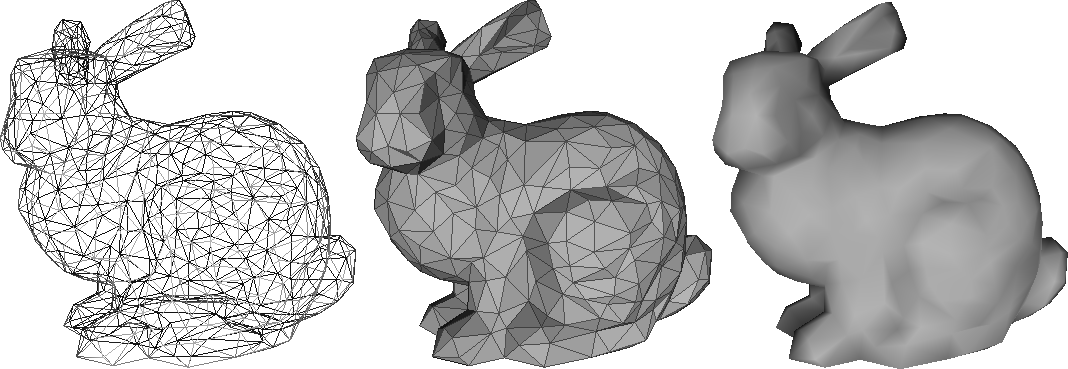
\includegraphics[width=1\textwidth]{bunny}
    
To compute the per-vertex normals you should first compute the per-face normals, and then average them on the neighboring vertices. In other words, the normal of the vertex of a mesh should be the average of the normals of the faces touching it. Remember to normalize the normals after averaging.

When an object is selected, it must be possible to switch between the different rendering modes by pressing three keys on the keyboard.

\subsection{Camera Control}

Add the possibility to translate the position of the camera (similarly to the previous assignment), but in this exercise the camera should always \emph{point to the origin}. It should be possible to move it around, but the camera should always face the origin.

Implement both a \emph{orthographic camera} (similar to the one that you used for Assignment 2, but in 3D) and a \emph{perspective camera}. The cameras should take into account the size of the window, properly adapting the aspect ratio to not distort the image whenever the window is resized. All functionalities should work after resizing the window, including object selection and editing of the scene.

\section*{Optional Tasks}

These tasks are optional. The first task is worth 2\% of the final grade, the second 3\%, and the third task 2\%. The optional points are added to the points of the other exercises, but the total sum of points that you gain with exercises cannot be more than 80\%.

\subsection{Animation Mode}

Add the possibility to draw a Bezier curve for each object in the scene. This should be done by having at least one key that allows to add a new control point and three keys to translate the point around. It is not necessary to have a UI that allows to edit the curve. Whenever the button space is pressed, each object should start to move following its associated curve, i.e. it's barycenter should follow the curve. The animation should last 5 seconds, and at the end all objects should go back to their previous state. The curve should be evaluated using De Casteljau's algorithm (See the course's textbook, pages 390-392).

\subsection{Export in SVG format}

Add the possibility to export the scene currently drawn on the screen in SVG format \url{https://en.wikipedia.org/wiki/Scalable_Vector_Graphics}. The exported SVG should be compatible with \url{https://inkscape.org/}. The triangles should be rendered only using flat shading and they should be deformed according to the current view (orthographic and perspective should both be supported). Hidden triangles should not be rendered (to check for hidden triangles, you can cast three rays to its vertices, and if any vertex is not visible you will simply skip the triangle).

\subsection{Trackball}

%\begin{wrapfigure}{r}{0.2\textwidth}
  \begin{center}
    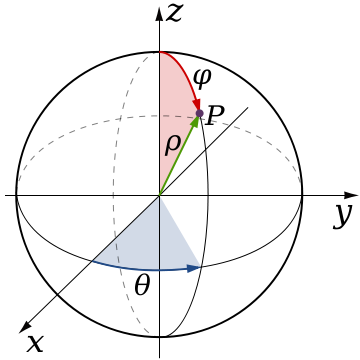
\includegraphics[width=0.5\textwidth]{trackball}
  \end{center}
%  \caption{Birds}
%\end{wrapfigure}
Use a trackball to control the camera. This can be achieved restricting the movement of the camera on a sphere centered on the origin. The easiest way to do it is to parametrize the sphere using spherical coordinates, and to assign keyboard keys to move the camera on the sphere. The camera should always look at the origin.




%\bibliographystyle{plain}
%\bibliography{bib.bib}
\end{document}  
